\documentclass[a4paper, 11pt]{article}
\usepackage{comment}
\usepackage{fullpage}
\usepackage{amsmath}
\usepackage{amssymb}
\usepackage{mathtools}
\usepackage{fontspec}
\defaultfontfeatures{Ligatures=TeX}
\usepackage{xfrac}
\usepackage{icomma}
\usepackage[section,below]{placeins}
\usepackage[labelfont=bf,font=small,width=0.9\textwidth]{caption}
\usepackage{subcaption}
\usepackage{graphicx}
\usepackage{grffile}
\usepackage{float}
\floatplacement{figure}{htbp}
\floatplacement{table}{htbp}
\usepackage{booktabs}
\usepackage{hyperref}
\usepackage[ngerman]{babel}
\begin{document}
\noindent
%\centerline{\small{\textsc{Technische Universität Dortmund}}} \\
\large{\textbf{4. Übungsblatt zur Vorlesung \hfill WS 2017/2018 \\
Statistische Methoden der Datenanalyse \hfill Prof. W. Rhode}} \\
Annika Burkowitz, Sebastian Bange, Alexander Harnisch \\
\noindent\makebox[\linewidth]{\rule{\textwidth}{0.4pt}}

\section*{Aufgabe 11: \normalfont{\textit{Simulationskette für Neutrinodetektor}}}
\subsection*{a) Signal MC}
Mit Hilfe der Transformationsmethode werden $10^5$ Signalereignisses des
Neutrinoflusses
\begin{equation}
  \Phi = \Phi_0 \left(\frac{E}{\text{TeV}}\right)^{-\gamma},
\end{equation}
mit $\gamma = 2.7$, erzeugt. Für die Transformationsmethode wird der Fluss zunächst
von $1\,\text{TeV}$ bis $E$ integriert und dann invertiert.
\begin{figure}
  \centering
  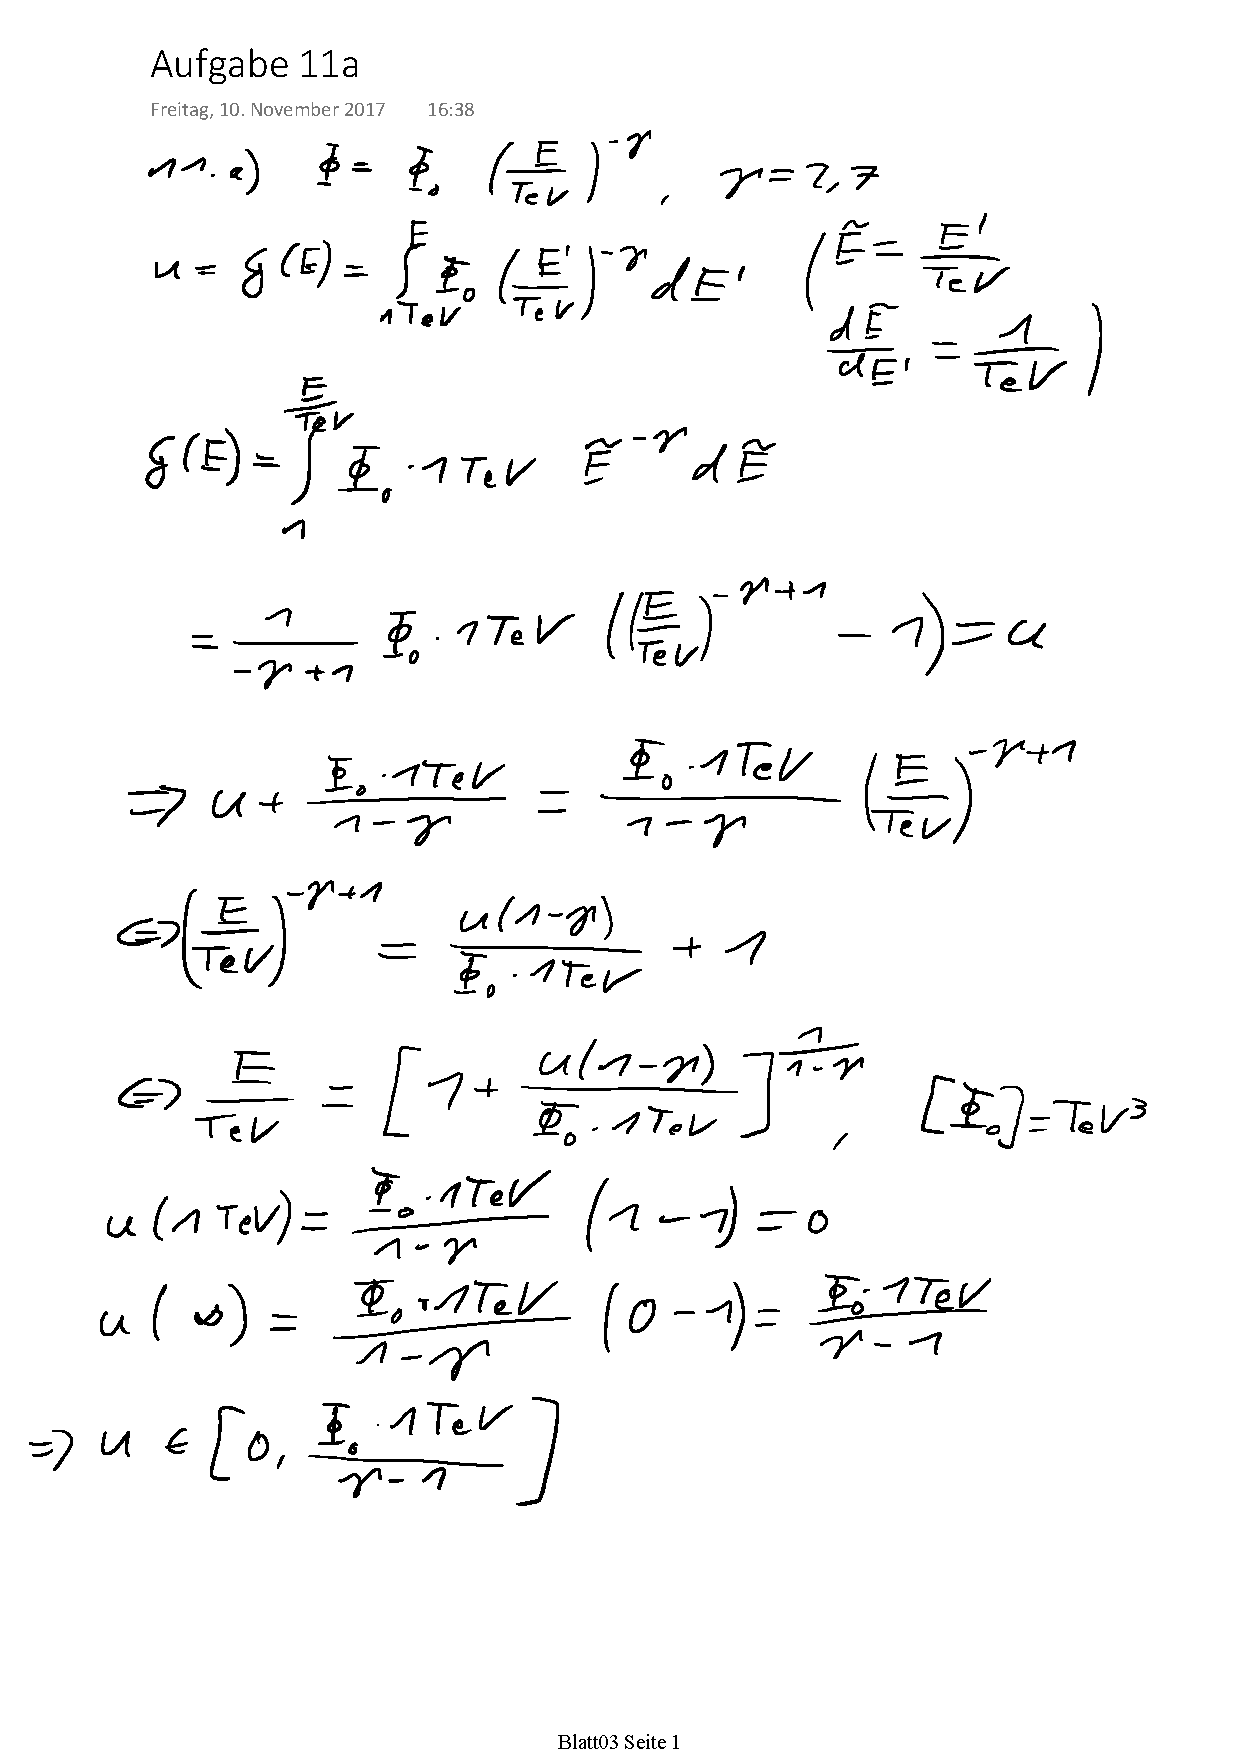
\includegraphics[width=\textwidth]{../A11/Rechnung.pdf}
\end{figure}
Das Ziehen von gleichverteilten Zufallszahlen $u$ im Intervall
$\lbrack 0, \frac{\Phi_0 \, 1\,\text{TeV}}{\gamma -1} \rbrack$ und Einsetzen in
\begin{equation}
  \frac{E}{1\,\text{TeV}}
  = \left(1+\frac{u (1-\gamma)}{\Phi_0\, 1\,\text{TeV}}\right)^{\frac{1}{1-\gamma}}
\end{equation}
liefert die gewünschten Signale. Diese werden in einem DataFrame mit dem Key
Energy abgespeichert.

\FloatBarrier
\subsection*{b) Akzeptanz}
Da die Detektionswahrscheinlichkeit energieabhängig ist, müssen die in Aufgabenteil
a) erzeugten Signale modifiziert werden.
Dazu wird für jede zuvor bestimmte Energie die Detektionswahrscheinlichkeit nach
der Gleichung
\begin{equation}
  P(E) = (1-e^{-E/2})^3
\end{equation}
bestimmt. Dann werden $10^5$ gleichverteilte Zufallszahlen $r$ zwischen 0 und 1
mit numpy.random.uniform() gezogen und es wird eine Maske erstellt, indem
elementweise verglichen wird, ob $r<P(E)$ gilt. Diese Maske wird in dem DataFrame
unter dem Key AcceptanceMask gespeichert.
In Abbildung \ref{fig:akzeptiertes-signal} sind die Histogramme der erzeugten und
der akzeptierten Signale überlagert doppelt-logarithmisch dargestellt. Der sichtbare
blaue Bereich entspricht dem Anteil des erzeugten Signals, der verworfen wird.
\begin{figure}
  \centering
  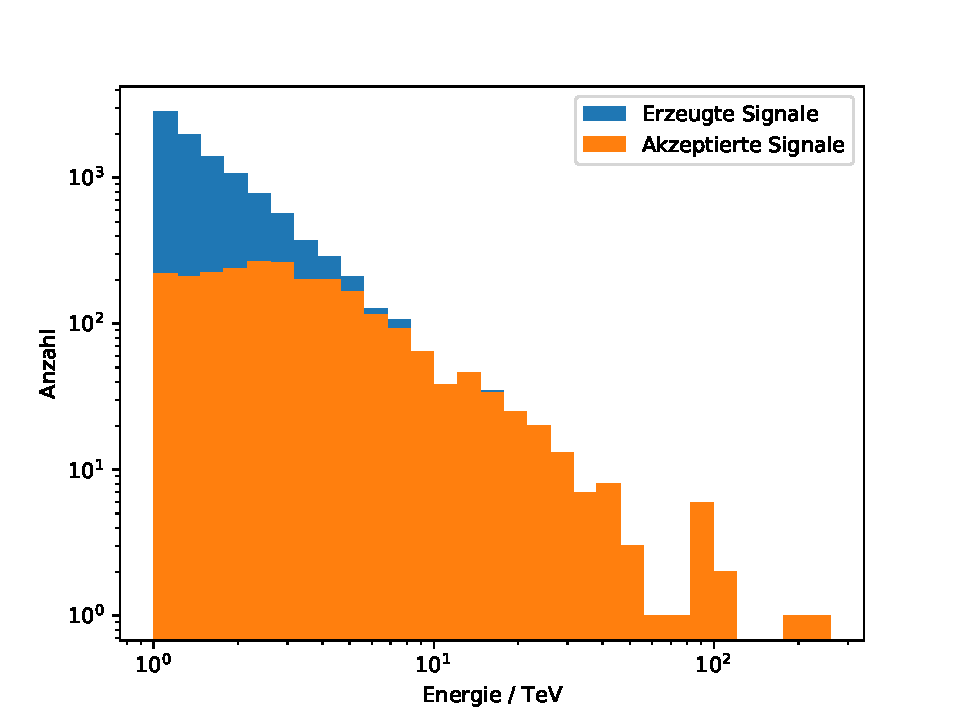
\includegraphics[width=\textwidth]{../A11/Energie.pdf}
  \caption{Histogramm der erzeugten und akzeptierten Signale. Aufgetragen ist die
  Energie gegen die Häufigkeit.}
  \label{fig:akzeptiertes-signal}
\end{figure}

\FloatBarrier
\subsection*{c) Energiemessung}
In diesem Aufgabenteil wird die Anzahl der Hits, also die Anzahl der Photomultiplier,
die angesprochen haben, für die akzeptierten Energien simuliert.
Dazu werden mit der Polarmethode eine normalverteilte Zufallszahlen mit dem
Mittelwert $10 E$ und der Standarabweichung $2E$ generiert.
% Polarmethode erklären?
Da die Anzahl der
Hits eine ganze, nicht negative Zahl sein muss, werden alle negativen Zufallszahlen
verworfen und die Anzahl wird auf eine ganze Zahl gerundet. Die Anzahl Hits wird
in dem DataFrame unter dem Key NumberOfHits gespeichert. Des Weiteren wird ein
Histogramm für die Hits erstellt, das in Abbildung \ref{fig:hits} zu sehen ist.
\begin{figure}
  \centering
  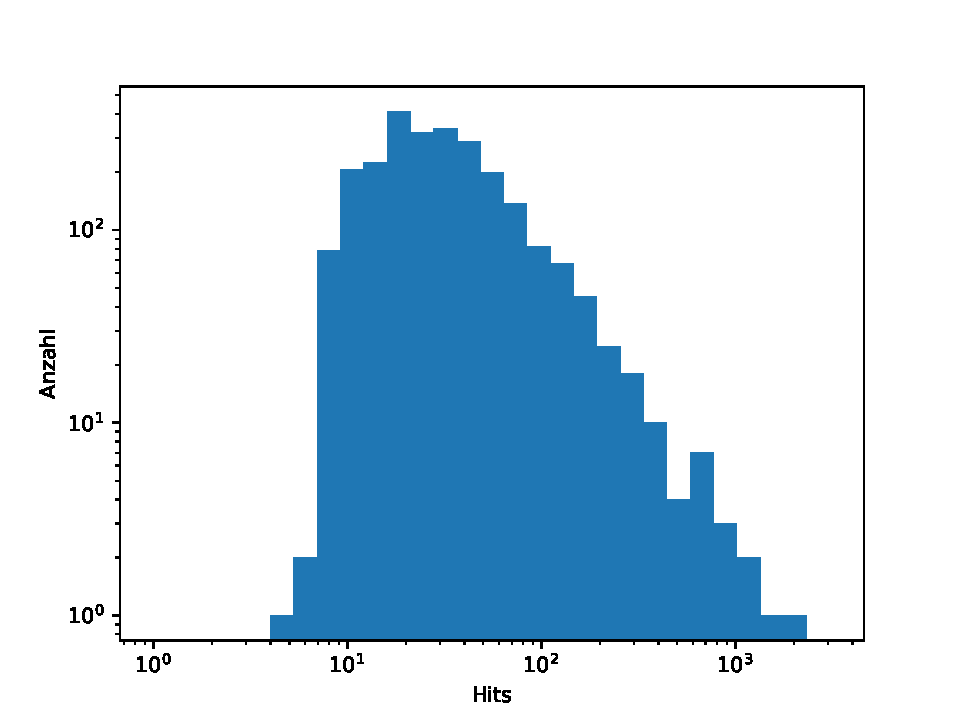
\includegraphics[width=\textwidth]{../A11/Hits.pdf}
  \caption{Histogramm für die Hits in Abhängigkeit der akzeptierten Energien.}
  \label{fig:hits}
\end{figure}

\FloatBarrier
\subsection*{d) Ortsmessung}
Es wird ein quadratischer Flächendetektor mit der Kantenlänge 10 Längeneinheiten
simuliert, bei dem im Punkt (7,3) das Signal auftrifft. Die energieabhängige
Ortsauflösung wird durch eine Normalverteilung in x-Richtung und eine Normalverteilung
in y-Richtung mit der Standardabweichung $\sigma = \left(\log_10(N+1)\right)^{-1}$
simuliert. Es gilt $\mu_\text{x}=7$ und $\mu_\text{y}=3$.
Gezogene Ergebnisse, die außerhalb der Fläche des Detektors liegen werden
verworfen und neu gezogen. Die Koordinaten der Orte werden mit den Keys x und y
im DataFrame gespeichert. Aus den erhaltenen Orten wird ein zweidimensionales
Histogramm erstellt, das in Abbildung \ref{fig:orte} dargestellt ist.
\begin{figure}
  \centering
  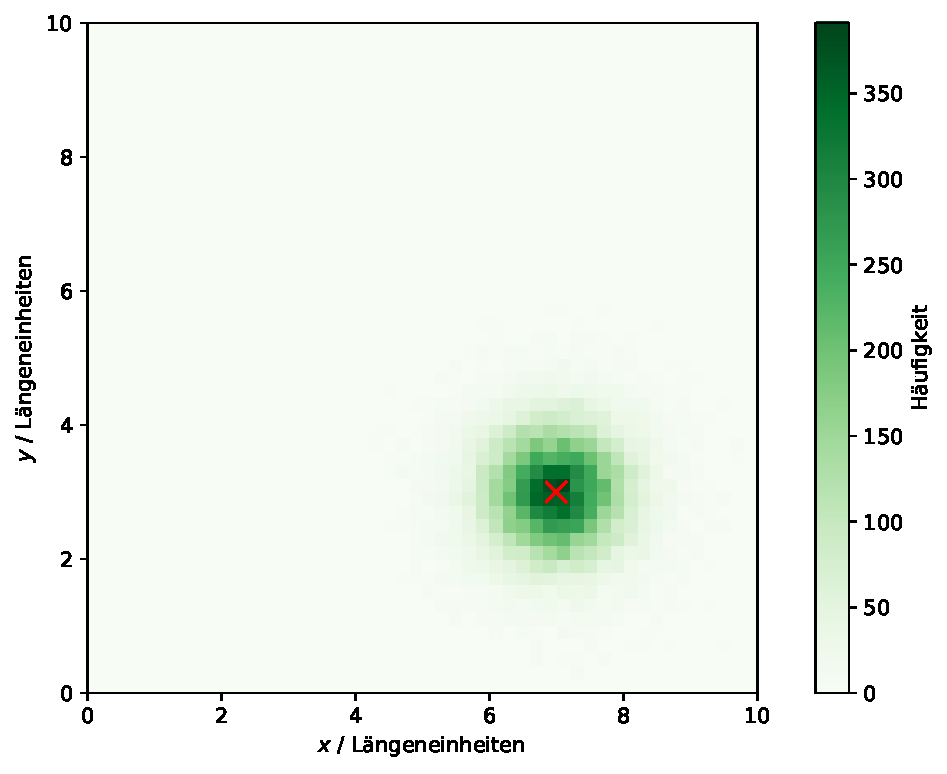
\includegraphics[width=0.75\textwidth]{../A11/Orte.pdf}
  \caption{Zweidimensionales Histogramm für die Orte, an denen das Signal detektiert
  wird.}
  \label{fig:orte}
\end{figure}

\FloatBarrier
\subsection*{e) Untergrund MC}
Zuletzt werden noch $10^7$ Untergrundereignisse simuliert. Der Zehner-Logarithmus
der Anzahl der Hits folgt dabei einer Normalverteilung mit $\mu = 2$ und $\sigma=1$,
die x- und y-Koordinate sind um den Mittelpunkt (5,5) normalverteilt und zwischen
x und y besteht eine Korrelation von $\rho=0.5$:
\begin{align}
  x &= \sqrt{1-\rho^2} \cdot \sigma \cdot x^\text{*} + \rho \cdot \sigma y^\text{*} + \mu\\
  y &= \sigma \cdot y^\text{*} + \mu \,.
\end{align}
Abbildung \ref{fig:orte-background} zeigt ein zweidimensionales Histogramm der
Orte der Untergrundereignisse und der Logarithmus der Anzahl der Hits ist in einem
eindimensionalen Histogramm in Abbildung \ref{fig:hits-background} dargestellt.
\begin{figure}
  \centering
  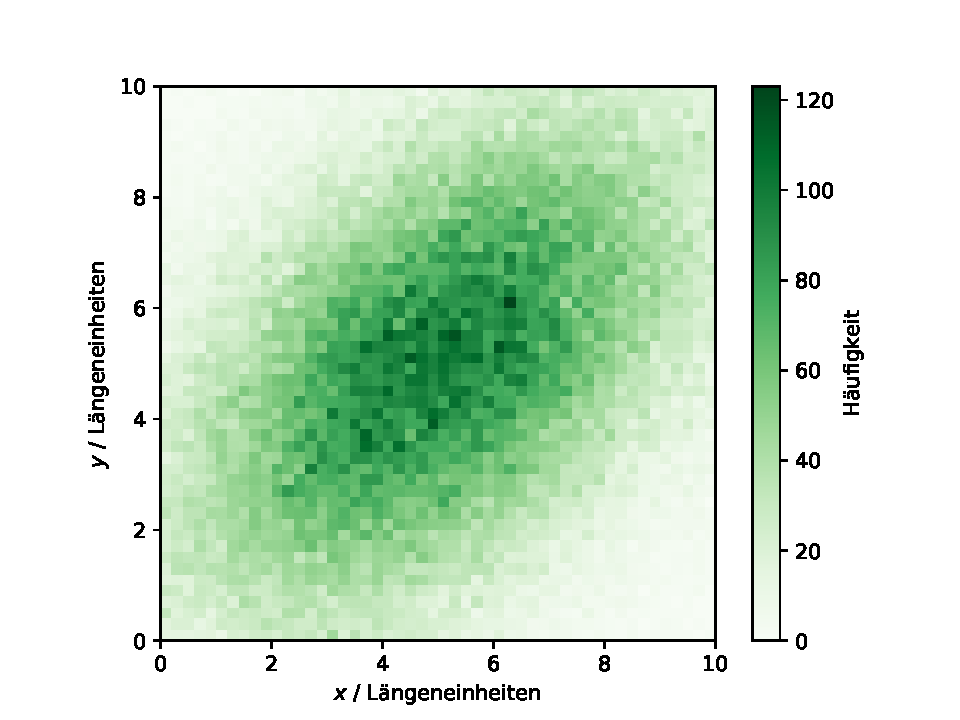
\includegraphics[width=0.75\textwidth]{../A11/OrteBackground.pdf}
  \caption{Zweidimensionales Histogramm der Orte der Untergrundereignisse.}
  \label{fig:orte-background}
\end{figure}
\begin{figure}
  \centering
  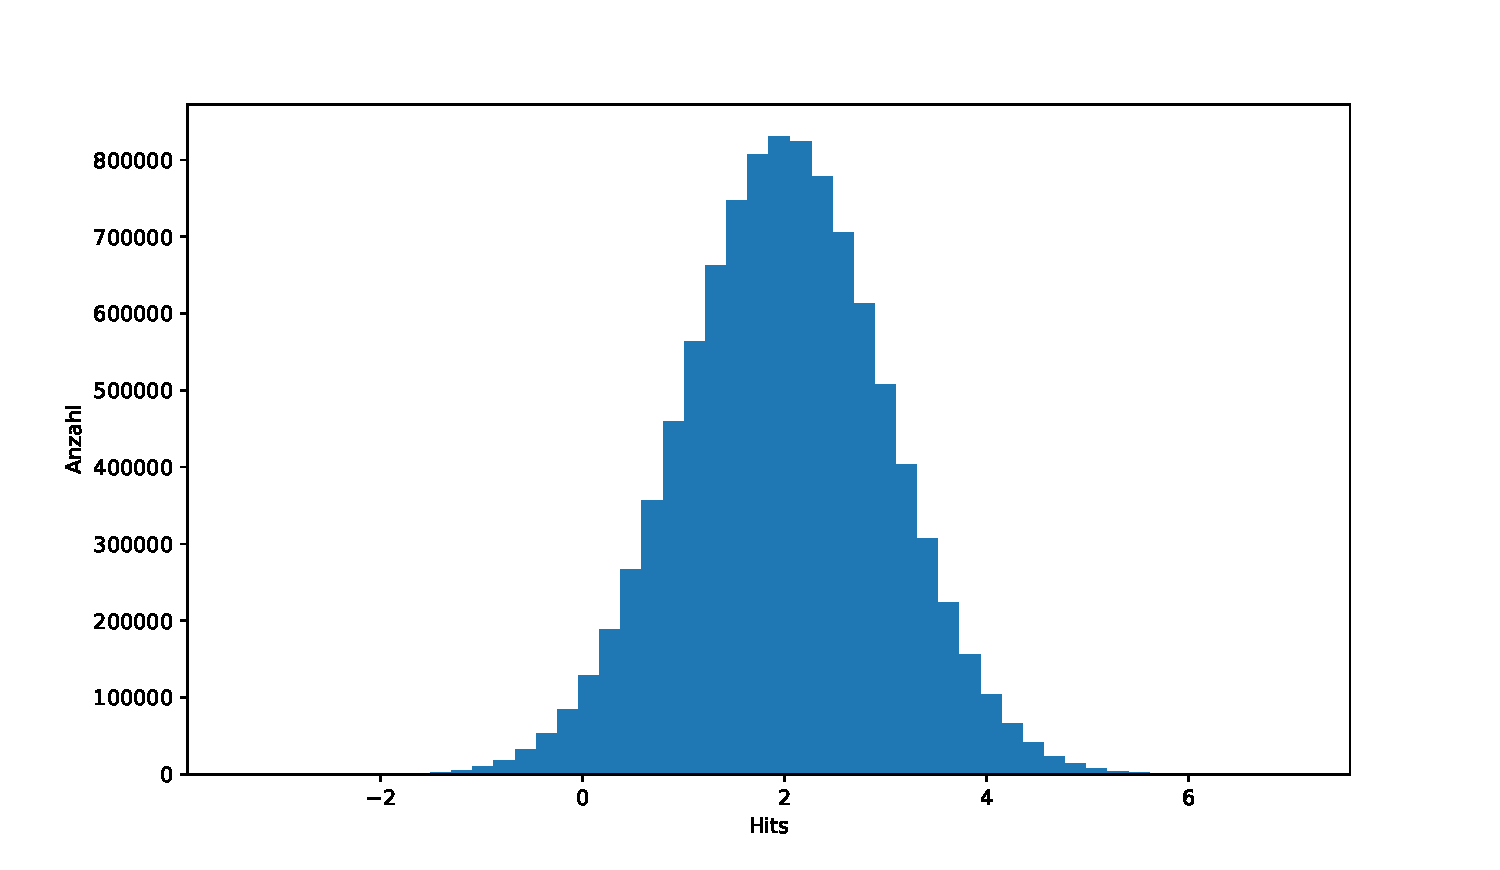
\includegraphics[width=\textwidth]{../A11/HitsBackground.pdf}
  \caption{Histogramm des Logarithmus der Anzahl der Hits des Untergrunds.}
  \label{fig:hits-background}
\end{figure}
\end{document}
